\documentclass{uebungszettel}

% Für die Verwendung von `diagrams` mit LaTeX
\usepackage[backend=cairo, outputdir=diagrams]{diagrams-latex}
\usepackage{graphicx}
\usepackage{tikz}

\begin{document}
\pagestyle{empty}

\maketitle{Klasse 8/9}{20. Januar 2017}

Im Leben und in der Mathematik (einem Teilgebiet des Lebens) kommt es häufig vor, dass aus~$n$ Personen/Sachen/Möglichkeiten $k$~Stück ausgewählt werden:

\begin{itemize}
  \item Ein Fußballtrainer muss vor einem Spiel aus seinen~$n$ Spielern eine Mannschaft von $k=11$ Spielern zusammenstellen.
  \item Beim Ausfüllen eines Lottoscheins muss man $k=6$ der $n=49$ Zahlen $1, \ldots, 49$ ankreuzen.
  \item Bei Familienfeiern stoßen alle Paare ($k=2$) von~$n$ Personen miteinander an.
  \item Beim Poker werden von den 52 verschiedenen Spielkarten in der ersten Runde drei Karten offen aufgedeckt.
\end{itemize}

Es stellt sich dabei die Frage, wie viele Möglichkeiten es jeweils gibt, die Fußballmannschaft zusammenzustellen, den Lottoschein auszufüllen, die ersten drei Karten aufzudecken bzw. wie oft beim Anstoßen die Gläser klirren.
Da solche Situationen häufig auftreten, haben Mathematiker sich dafür eine eigene Notation ausgedacht:
\[
  {n \choose k} \quad
  \text{}
\]
ist die Anzahl von Möglichkeiten, aus~$n$ Elementen $k$~Stück (ohne Beachtung der Reihenfolge) auszuwählen. Dieses Symbol wird "`$n$ über $k$"' ausgesprochen und \textit{Binomialkoeffizient} genannt.

Für kleine Zahlen~$k$ und~$n$ kann man alle Möglichkeiten auflisten und zählen. Zum Beispiel kann man so ${4 \choose 2} = 6$ oder ${4 \choose 3} = 4$ ausrechnen:

\begin{diagram}
import Diagrams.BinomialCoefficients
import qualified NiceColours as NC

dia =
  bcDiagram (simpleColourScheme NC.teal) 4 2
  ||| strutX 15 |||
  bcDiagram (simpleColourScheme NC.orange) 4 3
\end{diagram}

(Die Kreise mit buntem Rand stehen dabei für die ausgewählten Elemente.)

Für alle Zahlen $n$ ist ${n \choose 0} = 1$, denn es gibt nur eine Möglichkeit, keine Elemente auszuwählen (nämlich, kein Element auszuwählen).
Analog ist ${n \choose n} = 1$, denn wenn man alle Elemente auswählen soll, so hat man ebenfalls nur eine Möglichkeit.

Es gelten zahlreiche Gleichungen für die Binomialkoeffizienten.
Damit ist es möglich, Binomialkoeffizienten für große Zahlen~$n$ über~$k$ auszurechnen ohne alle Teilmengen aufzulisten und durch Vergessen oder Doppeltzählen Fehler zu machen.

\begin{aufgabe}{Symmetrie der Binomialkoeffizienten}
  Für alle $n \geq 0$ und $k \geq 0$ gilt
  \[
    {n \choose k} = {n \choose n-k}.
  \]
  Kannst du dies anhand des folgenden Diagramms (das $n = 5$ und $k = 3$ zeigt) beweisen?
  
\begin{diagram}
import Diagrams.BinomialCoefficients
import qualified NiceColours as NC

dia =
  bcSymmetryDiagram
    (ColourScheme { dotColour = black, selectionColour = NC.blue })
    (ColourScheme { dotColour = black, selectionColour = NC.green })
    5 3
\end{diagram}
\end{aufgabe}

\newpage

\begin{aufgabe}{Eine Rekursionsformel mit Addition}
  Für $n \geq 1$ und $k \geq 1$ gilt
  \[
    {n \choose k} = {n-1 \choose k-1} + {n-1 \choose k}.
  \]
  Kannst du dies mit dem folgenden Diagramm (welches $n = 6$ und $k = 4$ zeigt) beweisen?
  
\begin{diagram}
import Diagrams.BinomialCoefficients
import qualified NiceColours as NC

dia =
  bcAdditionIdentityDiagram
    (ColourScheme { dotColour = black, selectionColour = NC.teal })
    6 4
\end{diagram}
\end{aufgabe}

\begin{aufgabe}{Das Pascalsche Dreieck}
  Man kann die Binomialkoeffizienten in Form eines Dreiecks anordnen, wobei $n$ in jeder Zeile fest ist und $k$ von $0$ auf $n$ steigt.
  Diese Form heißt in Deutschland \emph{Pascalsches Dreieck} (nach dem frz. Mathematiker \textit{Blaise Pascal}, 1623-1662)\footnote{Im Iran ist das Dreieck als Khayyam-Dreieck (nach dem persischen Dichter-Astronomen-Mathematiker Omar Khayyám, 1048–1131) bekannt. In China ist es nach dem Mathematiker Yang Hui (ca. 1238–1298) benannt. In Italien heißt es Tartaglia-Dreieck (nach Niccolò Fontana Tartaglia, 1500–1577)}.
  
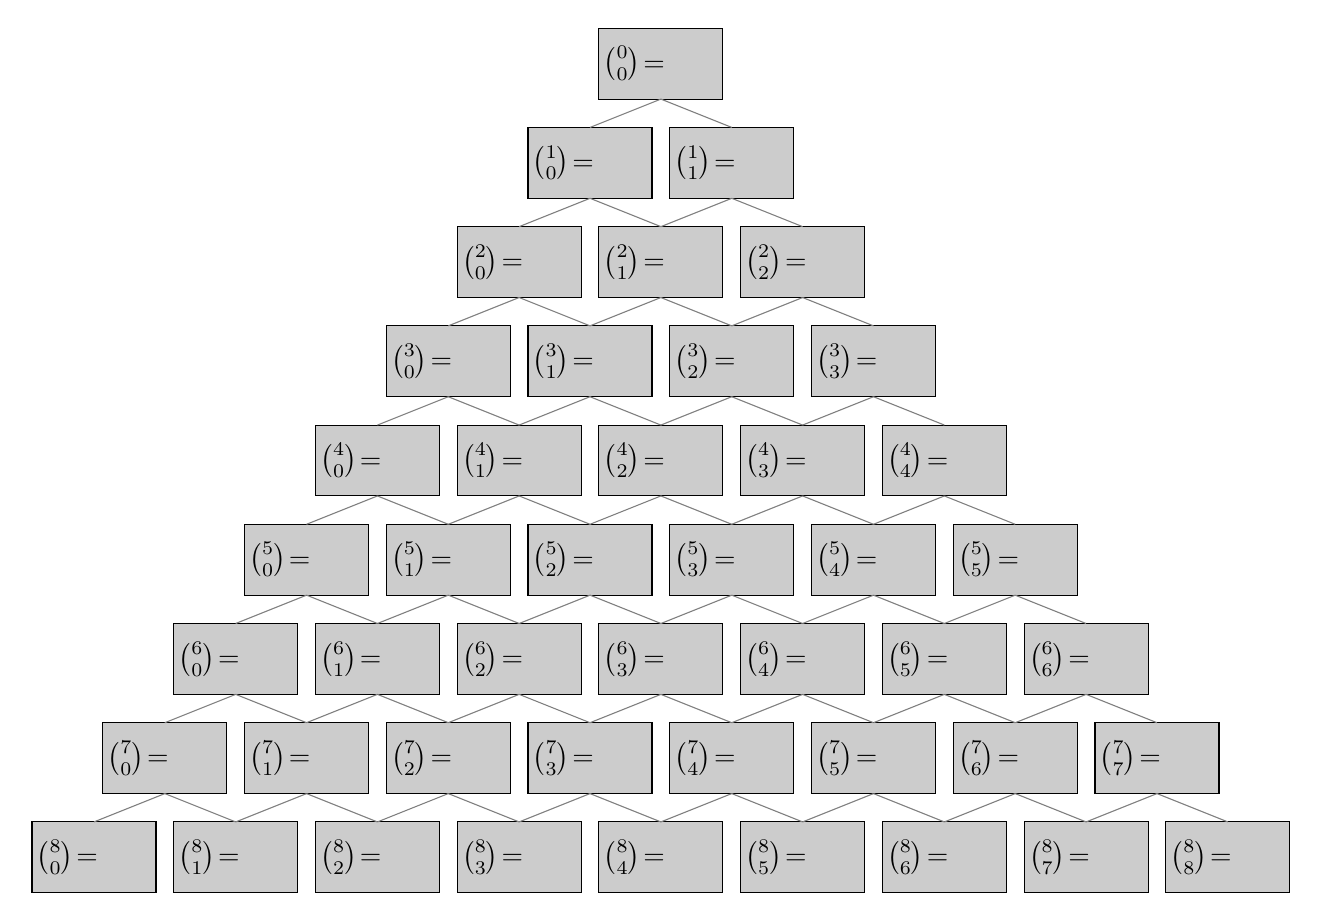
\begin{tikzpicture}[scale=0.9]
\foreach \n in {0,...,8} {
  \foreach \k in {0,...,\n} {
    \ifthenelse{\equal{\intcalcMod{2*\n-\k}{5}}{0}}{
      \def\fillcolor{red};
    }{
      \ifthenelse{\equal{\intcalcMod{2*\n-\k}{5}}{1}}{
        \def\fillcolor{green};
      }{
        \ifthenelse{\equal{\intcalcMod{2*\n-\k}{5}}{2}}{
          \def\fillcolor{blue};
        }{
          \ifthenelse{\equal{\intcalcMod{2*\n-\k}{5}}{3}}{
            \def\fillcolor{yellow};
          }{
            \def\fillcolor{orange};
          }
        }
      }
    }
    \draw [fill=\fillcolor, fill opacity=0.2] (2*\k - \n, -1.4*\n) rectangle + (1.75,1);
    \node at (2*\k - \n + 0.5, -1.4*\n + 0.5) {${\n \choose \k} \!=$};
  }
}
\foreach \n in {0,...,7} {
  \foreach \k in {0,...,\n} {
    \draw [gray] (2*\k - \n + 0.875, -1.4*\n) -- + (-1,-0.4);
    \draw [gray] (2*\k - \n + 0.875, -1.4*\n) -- + (1,-0.4);
  }
}
\end{tikzpicture}

\begin{itemize}
  \item[a)] Benutze die Rekursionsformel aus der letzten Aufgabe, um das Dreieck auszufüllen!
  \item[b)] Begründe folgende Aussage: \textit{Die Summe der Zahlen einer Zeile ist genau das Doppelte der Summe der Zahlen in der vorherigen Zeile.}
  
  Folgere: \textit{Die Summe der Zahlen der $n$-ten Zeile ist genau $2^{n-1}$.}
  \item[c)] Berechne die Summe der Zahlen in den farblich markierten, von links-oben nach rechts-unten verlaufenden Diagonalen. Was stellst du fest? Kannst du deine Beobachtung begründen?
\end{itemize}
\end{aufgabe}

\newpage

\begin{aufgabe}{Wege im Gitter}
  Ein Marienkäfer sitzt unten links in einem Gitter und möchte auf einem der kürzesten Wege zum Kleeblatt oben rechts laufen. Er kann sich dabei nur auf den Gitterlinien bewegen. Wie viele unterschiedliche Wege gibt es?
  
  \begin{center}
    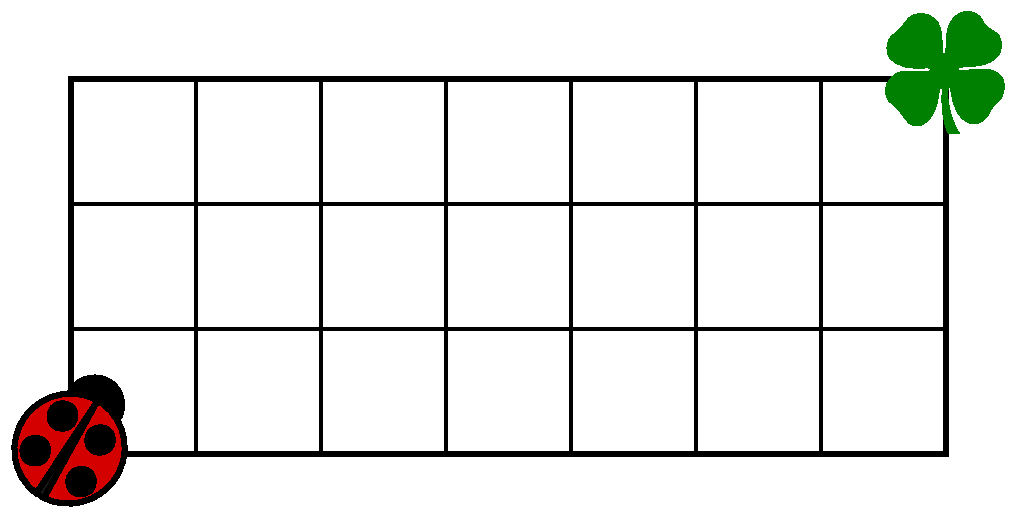
\includegraphics[scale=0.6]{ladybug-binomialcoefficients.pdf}
  \end{center}
\end{aufgabe}

\begin{aufgabe}{Eine Rekursionsformel mit Multiplikation}
  Für $n \geq 1$ und $k \geq 1$ gilt
  \[ k \cdot {n \choose k} = n \cdot {n-1 \choose k-1}. \]
  Das folgende Diagramm soll dies im Fall $n=5$ und $k=3$ zeigen: 
  $3 \cdot {5 \choose 3} = 5 \cdot {4 \choose 2}$.
  Kannst du den Beweis erklären?
  
\begin{diagram}
import Diagrams.BinomialCoefficients
import qualified NiceColours as NC

dia =
  bcMultiplicativeIdentityDiagram
    (ColourScheme { dotColour = black, selectionColour = NC.red })
    (ColourScheme { dotColour = NC.yellow, selectionColour = NC.red })
    5 3
\end{diagram}

{\footnotesize Tipp: Wie viele Möglichkeiten gibt es, aus~$n$ Spielern eine Mannschaft von~$k$ Spielern, darunter einen Kapitän, auszuwählen?}
\end{aufgabe}

\begin{aufgabe}{Sechser im Lotto}
  Aus der vorhergehenden Aufgabe folgt
  \[
    {n \choose k} = \frac{n}{k} \cdot {n-1 \choose k-1}
    \qquad \text{für alle $n \geq 1$ und $k \geq 1$.}
  \]
  Benutze diese Tatsache, um die Zahl ${49 \choose 6}$, die Anzahl der Kombinationen beim Lotto "`6aus49"', auszurechnen!
\end{aufgabe}

\newpage

\begin{aufgabe}{Summe verschobener Binomialkoeffizienten}
  Für alle $n \geq 0$ und $m \geq 0$ gilt die Gleichung
  \[
    {n+m+1 \choose n+1} = {n \choose n} + {n+1 \choose n} + \ldots + {n+m-1 \choose n} + {n+m \choose n}.
  \]
  Erkläre diese Gleichung mit der Skizze, die den Fall $n=2$ und $m=3$ zeigt!
  
\begin{diagram}
import Diagrams.BinomialCoefficients
import qualified NiceColours as NC

dia =
  shiftedBcsIdentityDiagram
    (simpleColourScheme NC.orange)
    2 3
\end{diagram}
\end{aufgabe}

\begin{aufgabe}{Vandermondesche Identität}
  Die \emph{Vandermondesche Identität} besagt, dass für alle~$m$, $n$ und~$k$ gilt:
  \[
    {m+n \choose k} = {m \choose 0} \cdot {n \choose k} + {m \choose 1} \cdot {n \choose k-1} + \ldots + {m \choose k-1} \cdot {n \choose 1} + {m \choose k} \cdot {n \choose 0}
  \]
  Für $m=4$, $n=3$ und $k=2$ gilt also
  \[
    {4+3 \choose 2} = {4 \choose 0} \cdot {3 \choose 2} + {4 \choose 1} \cdot {3 \choose 1} + {4 \choose 2} \cdot {3 \choose 0}.
  \]
  Warum gilt diese Gleichung?
  Das kannst du anhand der Abbildung für den Fall $m = 3$, $n = 4$, $k = 3$ nachvollziehen:

\begin{diagram}
import Diagrams.BinomialCoefficients
import qualified NiceColours as NC

dia =
  vandermondIdentityDiagram schemeM schemeN 3 4 3
  where
    schemeM = ColourScheme { dotColour = NC.green, selectionColour = NC.navy }
    schemeN = ColourScheme { dotColour = NC.red, selectionColour = NC.navy }
\end{diagram}
\end{aufgabe}

\begin{aufgabe}{Der binomische Lehrsatz}
  Zeige, dass für alle $n \geq 0$ gilt:
  \begin{align*}
    (x + y)^n & = \sum_{k=0}^n {n \choose k} \cdot x^k y^{n-k} \\
    & = {n \choose 0} \cdot x^0 y^n + {n \choose 1} \cdot x^1 y^{n-1} + \ldots + {n \choose n-1} \cdot x^{n-1} y^1 + {n \choose n} \cdot x^n y^0.
  \end{align*}
  {\footnotesize Tipp: Verwende das Distributivgesetz $(a + b) \cdot c = a \cdot c + b \cdot c$, um $(x + y)^n$ umzuschreiben als Summe von Produkten der Form $x^i \cdot y^j$. Zähle dann die Summanden mit gleichen Exponenten.}
\end{aufgabe}

\newpage

\begin{aufgabe}{Alternierende Summe von Binomialkoeffizienten}
  Für alle natürlichen Zahlen~$n$ gilt:
  \[
    {n \choose 0} - {n \choose 1} + {n \choose 2} - \ldots \pm {n \choose n-1} \mp {n \choose n} = 0
  \]
  Dabei addiert man alle Zahlen ${n \choose k}$ mit~$k$ gerade und subtrahiert von dieser Summe alle Zahlen ${n \choose k}$ mit $k$~ungerade.
  Erkläre folgenden Beweis ohne Worte für diese Gleichung!

\begin{center}
\begin{diagram}
import Diagrams.BinomialCoefficients
import qualified NiceColours as NC

dia =
  alternatingBcsIdentityDiagram (simpleColourScheme NC.lime) 6
    # center
    # rotateBy (-0.25)
    # scale 0.8
\end{diagram}
\end{center}

{\footnotesize Tipp: Drehe das Blatt um 90 Grad nach links. Wie viele Fünfer-Cliquen sind in jeder Spalte? Wann sind zwei Cliquen verbunden? Es kann hilfreich sein, die fünf Kreise jeder Clique durchzunummerieren von eins bis fünf, angefangen beim obersten Kreis.}
\end{aufgabe}

\end{document}